\documentclass[aspectratio=169,usenames,dvipsnames]{beamer}
\usepackage{preamble}
\title{Coding for Humanities, week 2}
\begin{document}

\begin{frame}
 \titlepage
\end{frame}

\begin{frame}{Plan for today}
 \tableofcontents
\end{frame}

\section{Strings}
\frame{\tableofcontents[currentsection]}

\begin{frame}{Strings}
    \begin{definition}
        A \structure{string}, short for string of characters,
        is a type of value that contains text.
    \end{definition}

\end{frame}

\begin{frame}[fragile]{Operations on strings}
\begin{lstlisting}
>>> first = 'John'
>>> last = 'Doe'
\end{lstlisting}
\begin{description}
    \item[first + last] \texttt{'JohnDoe'}
    \item[first - last] TypeError
    \item[first * last] TypeError
    \item[first / last] TypeError
\end{description}

\begin{itemize}
\item + can be used to concatenate two strings
\item The other operations require numbers, not text
\end{itemize}
\end{frame}

\begin{frame}[fragile]{Mixing strings and numbers}
\begin{lstlisting}
>>> first = 'John'
>>> num = 3
\end{lstlisting}
\begin{description}
    \item[first + num] TypeError
    \item[first - num] TypeError
    \item[first * num] 'JohnJohnJohn'
    \item[first / num] TypeError
\end{description}

\begin{itemize}
\item * can be used to repeat a string several times
\item For the other operations, Python refuses to mix up types
\end{itemize}
\end{frame}


\begin{frame}[fragile]{Indexing}
\begin{lstlisting}
>>> name = 'John'
>>> name[0]
'J'
>>> name[-1]
'n'
\end{lstlisting}
    \begin{itemize}
        \item a[n] gets the n'th character of a
        \item Counting starts at 0
        \item negative indices start from the end:\\
			-1 for last character, \\
            -2 second to last, etc.
    \end{itemize}
\end{frame}

\begin{frame}[fragile]{Slicing}
\begin{lstlisting}
>>> name = 'John'
>>> name[1:3]
'oh'
\end{lstlisting}
    \begin{itemize}
        \item a[n:m] extracts characters n to m
        \item Counting starts at 0
        \item Result is up to but not including character m
    \end{itemize}
\end{frame}

\begin{frame}[fragile]{Slicing shortcuts}
\begin{lstlisting}
>>> name = 'John'
>>> name[:2]
'Jo'
>>> name[1:]
'ohn'
\end{lstlisting}
    \begin{itemize}
        \item if n or m is left out, beginning or end is used
    \end{itemize}
\end{frame}

\begin{frame}[fragile]{Length}
\begin{lstlisting}
>>> name = 'John'
>>> len(name)
4
\end{lstlisting}
\end{frame}

\begin{frame}{Sequences}
    Strings are a kind of \structure{sequence}
    consisting of characters.

    A sequence contains elements in a particular order

    Several operations are supported:
    \begin{itemize}
        \item indexing:                    string[expression]
        \item slicing:                     string[start:end]
        \item concatenation:               string1 + string2
        \item repetition:                  string * expression
        \item getting length:              len(string)
    \end{itemize}
\end{frame}


\section{Lists}
\frame{\tableofcontents[currentsection]}

\begin{frame}[fragile]{Lists}
    \begin{definition}
    Lists are sequences that may contain any kind of value as items
    \end{definition}
\begin{lstlisting} 
>>> numbers = [0, 1, 2]
>>> names = ['John', 'Mary']
\end{lstlisting} 
\end{frame}

\begin{frame}[fragile]{Changing items}
\begin{lstlisting} 
>>> names = ['John', 'Mary']
>>> names[1] = 'Maria'
>>> names
['John', 'Maria']
\end{lstlisting} 

\pause
NB: cannot change characters in a string (must make new string)
\begin{lstlisting} 
>>> name = 'Maria'
>>> name[0] = 'D'
[...] TypeError: 'str' object does not support item assignment
\end{lstlisting}

Lists are mutable, strings are immutable:
\begin{definition}
An \structure{immutable} object cannot be changed after it is created.
\end{definition}
\end{frame}

\begin{frame}{Why immutable vs mutable?}
    \begin{description}
        \item[Immutable]
            \begin{itemize}
                \item Easier to reason about
                \item Constant values sometimes required
            \end{itemize}

        \item[Mutable]
            \begin{itemize}
                \item More efficient with many changes
                \item More natural
            \end{itemize}
    \end{description}
\end{frame}

\begin{frame}{Objects, methods}
    In Python, every value is an object:

    \begin{definition}
        An \structure{object} encapsulates
        data and code for dealing with that data.

        A function that belongs to and operates on an object
        is called a \structure{method}.
    \end{definition}
    
    Regular function: \texttt{f(a)}

    Method: \texttt{o.f(a)}
\end{frame}

\begin{frame}[fragile]{Adding items}
We can add an item to the end of an existing list:
\begin{lstlisting} 
>>> names = ['John', 'Mary']
>>> names.append('Alice')
['John', 'Mary', 'Alice']
\end{lstlisting}

\pause
We can combine two lists into a new list:
\begin{lstlisting} 
>>> friends = ['John', 'Mary']
>>> enemies = ['Alice', 'Bob']
>>> friends + enemies
['John', 'Mary', 'Alice', 'Bob']
\end{lstlisting}
\end{frame}


\begin{frame}[fragile]{Removing items}
We can remove an item anywhere in a list:
\begin{lstlisting} 
>>> names = ['John', 'Mary']
>>> names.remove('John')
['Mary']
\end{lstlisting}

    remove(elem) searches for the first occurrence of elem
    and removes it.

\pause
We can also use slicing to keep a part of a list
\begin{lstlisting} 
>>> acquaintances = ['John', 'Mary', 'Alice', 'Bob']
>>> friends = acquaintances[:2]
>>> friends
['John', 'Mary']
\end{lstlisting}

This is faster if you know where the items are that you want to keep.
\end{frame}


\begin{frame}[fragile]{The split method}
We can turn a string into a list of strings
by splitting on a character:
\begin{lstlisting} 
>>> quote = "Frankly, my dear, I don't give a damn."
>>> quote.split(",")
['Frankly', ' my dear', " I don't give a damn."]
\end{lstlisting}

\pause
If we don't give a character, splits on whitespace:
\begin{lstlisting} 
>>> quote.split()
['Frankly,', 'my', 'dear,', 'I', "don't", 'give', 'a', 'damn.']
\end{lstlisting}
\end{frame}


\begin{frame}[fragile]{Sorting}
\begin{lstlisting} 
>>> letters = ['o', 'c', 'd']
>>> sorted(letters)
['c', 'd', 'o']
\end{lstlisting}

NB: sorted leaves the original list unchanged,
assign it to keep the result.
\end{frame}

\begin{frame}[fragile]{Summary}
Python strings versus Python lists:

Both Python strings and lists are sequences and behave in very similar ways

Except for two important differences:
\begin{enumerate}
\item lists are more general data types than strings

    Strings always consist of characters

    Lists can consist of any data types / objects

\item lists are mutable and strings are immutable
\end{enumerate}
\end{frame}



\section{Dictionaries}
\frame{\tableofcontents[currentsection]}

\begin{frame}
    \begin{itemize}
        \item Lists are useful when data has a natural order: \\
            items are referred by their position
        \pause
        \item What if we have lots of data,
            but we need to find it some other way?
    \end{itemize}

    \begin{block}{Example}
    Finding words in a dictionary

    Too many words to consider one-by-one

    However, due to organization (sorted), can find words quickly
    \end{block}
\end{frame}


\begin{frame}[fragile]{dictionaries}
    \begin{definition}
        A dictionary stores pairs of values (key, value),
        such that we can quickly find a value given a key.
    \end{definition}
Example, a phone book:
\begin{lstlisting}
>>> coworkers = {'John': 123, 'Mary': 456, 'Alice': 789}
>>> coworkers['Mary']
456
>>> coworkers['Bob'] = 124
\end{lstlisting}

% Explanation of hash tables:
% https://dev.to/a_sandrina_p/learning-hash-tables-with-drawings-99o
\end{frame}

\begin{frame}{Properties of dictionaries}
A dictionary is a mapping of keys to values.

    \begin{itemize}
        \item Looking up a key is fast
        \item Keys must be immutable (e.g., numbers or strings).
        \item Values can be anything.
        \item Keys are always unique;
            re-using a key will overwrite the previous value.
    \end{itemize}
\end{frame}



\section{Data organization}
\frame{\tableofcontents[currentsection]}

\begin{frame}[fragile]{Combining lists and dictionaries}
Lists and dictionaries can contain any kind of value

Even other lists and dictionaries!

\begin{lstlisting}
>>> x = [[0, 1], [2, 3]]
>>> x[0]
[0, 1]
>>> x[0][0]
[0]
\end{lstlisting}
\end{frame}

\begin{frame}[fragile]{Practical example}
Two ways of organizing a collection of books:
\begin{lstlisting}
>>> books = ['Tolstoy - War and Peace', 'Tolstoy - Anna Karenina',
...     'Dostoevsky - Crime and Punishment',
...     'Dostoevsky - Brothers Karamazov']
\end{lstlisting}

\pause
\begin{lstlisting}
>>> books = {'Tolstoy': ['War and Peace', 'Anna Karenina'],
...     'Dostoevsky': ['Crime and Punishment',
...         'Brothers Karamazov']}
>>> books['Tolstoy']
...
\end{lstlisting}
The latter has the advantage of easily being able to
select the works by a particular author.
\end{frame}

\begin{frame}{Algorithms + Data structures = Programs}
    \begin{columns}
        \column{0.5\linewidth}
            \begin{itemize}
                \item Thinking of how to organize your data is an important
                    first step in designing a program
                \item The right organization may make the rest of the design
                    obvious
                \item Often a trade-off: particular choices may make one thing
                    easy and another hard
            \end{itemize}
        \column{0.5\linewidth}
            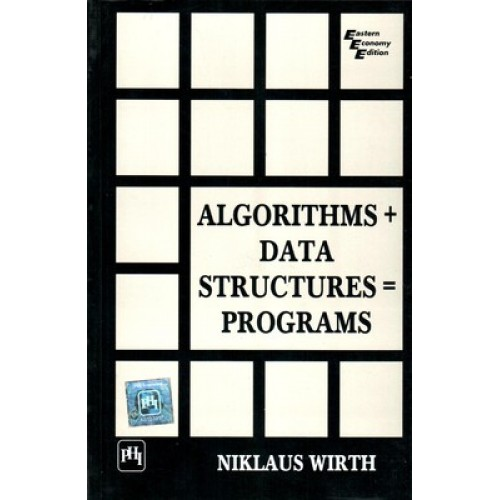
\includegraphics[height=0.8\textheight]{fig/wirth}
    \end{columns}
\end{frame}


\end{document}
